\documentclass[11pt,a4paper]{article}

\usepackage[utf8]{inputenc}
\usepackage[T1]{fontenc}
\usepackage[spanish]{babel}

\usepackage{tgpagella}
\usepackage{geometry}
\usepackage{booktabs}
\usepackage{xcolor}
\usepackage{graphicx}
\usepackage{titlesec}
\usepackage{fancyhdr}
\usepackage[parfill]{parskip}
\usepackage[expansion=false]{microtype}
\usepackage{hyperref}
\usepackage{setspace}
\usepackage{needspace}
\usepackage{etoolbox}
\usepackage{ragged2e}

\widowpenalty=10000
\clubpenalty=10000
\displaywidowpenalty=10000

\hyphenpenalty=8000
\exhyphenpenalty=8000

\geometry{top=3.0cm,bottom=3.0cm,left=3.5cm,right=3.5cm}

\setlength{\parskip}{0.65em}
\setlength{\parindent}{0em}

\definecolor{azulai}{RGB}{30,80,140}
\definecolor{doradoai}{RGB}{140,90,0}
\definecolor{grisai}{RGB}{70,70,70}

\AtBeginDocument{\RaggedRight}
\setlength{\rightskip}{0pt plus 2em}

\titleformat{\section}
{\Large\bfseries\color{azulai}\raggedright}
{}
{0em}
{}
[{\color{azulai}\titlerule[0.5pt]}]

\titlespacing*{\section}
{0pt}{1.3em}{0.5em}

\titleformat{\subsection}
{\large\bfseries\color{doradoai}\raggedright}
{}
{0em}
{}

\titlespacing*{\subsection}
{0pt}{1.0em}{0.35em}

\titleformat{\subsubsection}
{\normalsize\bfseries\color{grisai}\raggedright}
{}
{0em}
{}

\titlespacing*{\subsubsection}
{0pt}{0.8em}{0.25em}

\preto\section{\Needspace{8\baselineskip}}
\preto\subsection{\Needspace{6\baselineskip}}
\preto\subsubsection{\Needspace{4\baselineskip}}

\pagestyle{fancy}
\fancyhf{}

\rhead{\textcolor{grisai}{\small Izas — Arquitectura Interna}}
\lhead{\textcolor{grisai}{\small Mercurio · Venus · Marte}}
\cfoot{\textcolor{grisai}{\small\thepage}}

\renewcommand{\headrulewidth}{0.3pt}

\hypersetup{
colorlinks=true,
linkcolor=azulai,
urlcolor=azulai
}

\setstretch{1.32}

\tolerance=1500
\emergencystretch=4em

\begin{document}

% ── Portada ──────────────────────────────────────────────────────────────────

\begin{titlepage}
  \centering

  \vspace*{2cm}

  {\Huge\bfseries\color{azulai} Mercurio · Venus · Marte}\\[0.6cm]

  {\large\color{grisai} Arquitectura Interna}\\[0.4cm]

  {\small\itshape\color{grisai}
  Procesamiento, vínculo y acción en el funcionamiento cotidiano
  }\\[2.2cm]

  {\huge\color{doradoai} Izas}\\[1.6cm]

  {\Large 16/04/1979 \quad 04:20}\\[0.35cm]

  {\Large Pamplona, España}\\[0.35cm]

  {\normalsize
  Lat: 42.8157° \quad
  Lon: -1.6522° \quad
  UTC+02:00
  }\\[0.35cm]

  {\normalsize
  Ascendente: Acuario 6°20'
  \quad
  MC: Escorpio 29°12'
  }\\[2.2cm]

  \renewcommand{\arraystretch}{1.35}

  \begin{tabular}{ll}
    \textbf{Mercurio:} & Piscis — Casa 2 28°57' \\
    \textbf{Venus:}    & Piscis — Casa 1 21°30' \\
    \textbf{Marte:}    & Aries — Casa 2 7°01' \\
  \end{tabular}

  \vfill

  {\small\color{grisai}
  Generado el 19/05/2026
  }

\end{titlepage}

\RaggedRight

\tableofcontents

\clearpage

% ── Datos de referencia ───────────────────────────────────────────────────────
\section{Datos de referencia}

\begin{center}
\renewcommand{\arraystretch}{1.25}
\begin{tabular}{llll}
  \toprule
  \textbf{Planeta} & \textbf{Signo} & \textbf{Casa} & \textbf{Posición} \\
  \midrule
  Mercurio  & Piscis  & 2  & 28°57' \\
  Venus    & Piscis & 1 & 21°30' \\
  Marte    & Aries & 2 & 7°01' \\
  Ascendente          & Acuario           & ---                    & 6°20' \\
  Medio Cielo         & Escorpio            & ---                    & 29°12' \\
  \bottomrule
\end{tabular}
\end{center}
\RaggedRight

\vspace{0.5cm}

\textbf{Aspectos entre planetas personales:}

\begin{center}
\begin{tabular}{lllll}
  \toprule
  \textbf{Planeta 1} & \textbf{Asp.} & \textbf{Planeta 2} & \textbf{Tipo} & \textbf{Orbe} \\
  \midrule
  Mercurio & conj & Venus & Conjunción & 7.5° \\
  Mercurio & conj & Marte & Conjunción & 8.1° \\
  \bottomrule
\end{tabular}
\end{center}

\RaggedRight

\vspace{0.7cm}

\begin{center}
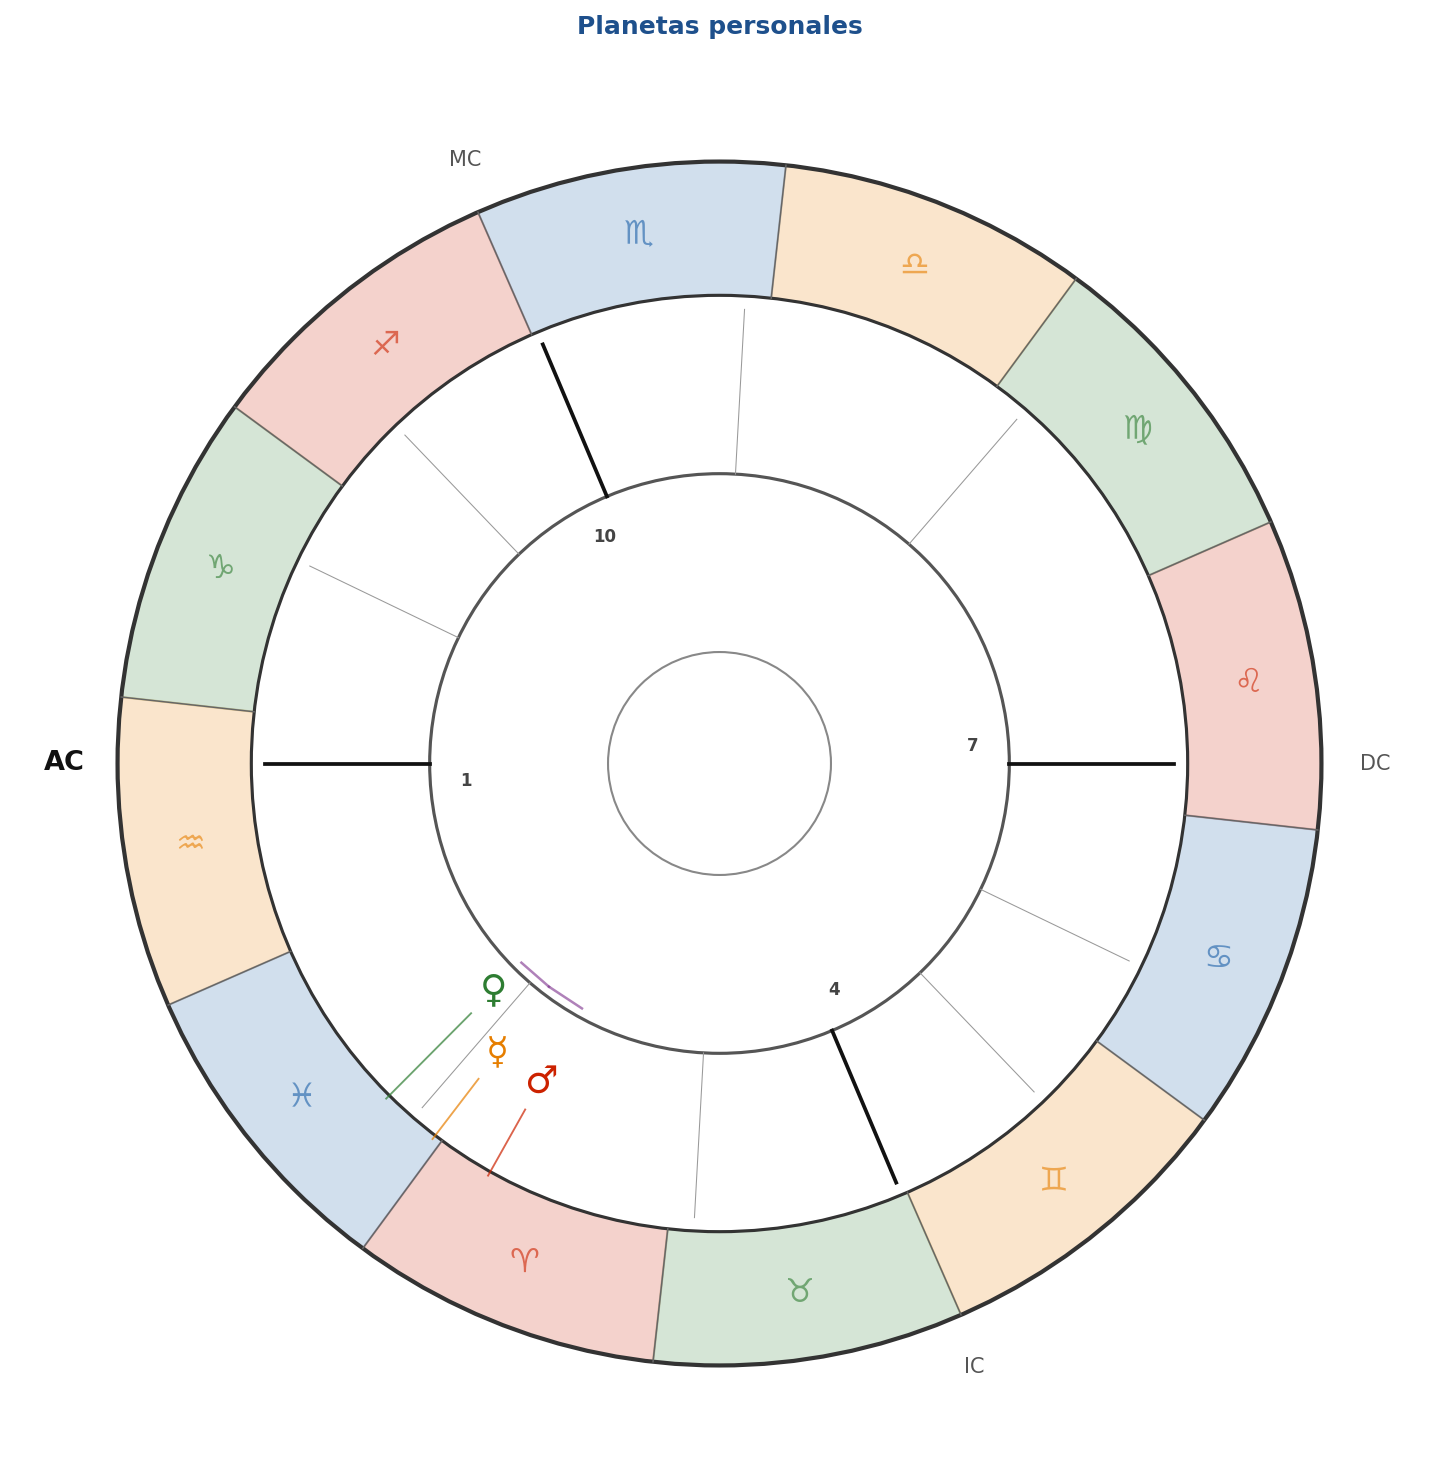
\includegraphics[width=0.72\textwidth]{Izas_Planetas_Personales_rueda.png}
\end{center}

\vspace{0.3cm}
\Needspace{5\baselineskip}

% ── Interpretación ────────────────────────────────────────────────────────────
\section{Interpretación — Arquitectura Interna}

\begin{center}
{\small\itshape\color{grisai}
No se trata de describir la personalidad.\\
Se trata de observar cómo procesas, cómo te vinculas\\
y cómo se mueve tu energía en la vida cotidiana.
}
\end{center}

\RaggedRight

\vspace{0.8cm}

% ── 1. Funcionamiento general ─────────────────────────────────────────────────
\subsection{1. Funcionamiento general}

\RaggedRight
Mercurio está en Piscis, Casa 2: muestra cómo piensas, cómo ordenas lo que percibes y cómo traduces lo que ocurre en palabras o ideas.
Venus está en Piscis, Casa 1: muestra cómo te vinculas, qué necesitas para sentir conexión y cómo buscas equilibrio afectivo.
Marte está en Aries, Casa 2: muestra cómo se activa tu acción, cómo descargas energía y cómo respondes ante el impulso.

Hay una concentración funcional de planetas personales: Mercurio, Venus, Marte. Esto indica que pensamiento, vínculo y acción no funcionan como partes aisladas, sino como un mismo campo de experiencia. Esta concentración se expresa en Aries, Piscis, en las casas 2, 1.

Cuando una de estas áreas se activa, las otras suelen responder rápidamente. Lo que piensas puede afectar a la forma en que te vinculas; lo que ocurre en tus relaciones puede modificar tu energía disponible; y la acción puede cambiar con rapidez la manera en que entiendes lo que estás viviendo. La ventaja es intensidad, coherencia interna y capacidad de respuesta. El riesgo es que, bajo presión, una sola área desorganizada arrastre a las demás.

Hay coherencia elemental entre: tu forma de pensar (Mercurio) y tu forma de vincularte (Venus) comparten elemento: Agua. Esto facilita que esas áreas colaboren entre sí. Aun así, lo que fluye con facilidad también puede volverse automático si no lo observas con consciencia.

Hay tensión elemental entre: tu forma de pensar (Mercurio, Agua) y tu forma de actuar (Marte, Fuego); tu forma de vincularte (Venus, Agua) y tu forma de actuar (Marte, Fuego). Esto no es un problema en sí mismo, pero sí pide más atención. Cuando esas áreas necesitan cooperar, conviene hacer una integración consciente para que una no bloquee, desborde o desconecte a la otra.

Hay conjunción entre planetas personales: Mercurio–Venus en conjunción (orbe 7.46°), Mercurio–Marte en conjunción (orbe 8.07°). Una conjunción une dos funciones de forma muy estrecha. No se vive como una simple relación entre partes separadas, sino como una mezcla interna: esas áreas tienden a encenderse juntas y a responder como una unidad.

\vspace{0.8cm}

% ── 2. Mercurio ───────────────────────────────────────────────────────────────
\subsection{2. Mercurio — Pensamiento y procesamiento}

\subsubsection*{Mercurio en Piscis — Casa 2}

\RaggedRight
Tu mente funciona de forma intuitiva y no lineal. Sueles percibir relaciones, ambientes y significados antes de poder explicarlos con claridad. Muchas veces entiendes algo primero como sensación, imagen o intuición, y solo después aparecen las palabras.

La saturación aparece cuando el entorno emocional es muy denso o confuso. Entonces absorbes demasiado y pierdes claridad sobre qué pensamientos son realmente tuyos y cuáles vienen del ambiente. El bloqueo suele aparecer como dificultad para concretar: hay percepción y sensibilidad, pero cuesta transformar todo eso en algo claro y utilizable.

Sueles pensar mejor cuando hay silencio, descanso mental, espacios de imaginación y tiempo para ordenar lo que percibes sin presión.

Tiendes a organizar la información de forma práctica, estable y gradual. Necesitas sentir que lo que aprendes tiene valor real, aplicación o utilidad concreta. Las ideas suelen asentarse lentamente, pero cuando lo hacen permanecen.

La saturación aparece cuando hay demasiada teoría sin aplicación o cambios constantes que no te dejan consolidar una comprensión estable. Sueles pensar mejor cuando puedes ir a tu ritmo y relacionar las ideas con experiencias reales y sostenibles.

En relación con los otros planetas personales:

Mercurio y Venus en conjunción: tu forma de pensar y tu forma de vincularte funcionan a través del mismo circuito. Necesitas comprender para conectar y muchas veces conectas a través de la conversación, las palabras y el intercambio mental.

Hablar, explicar y compartir ideas puede generar sensación real de cercanía. La dificultad aparece cuando analizar el vínculo reemplaza a vivirlo. Entonces la relación puede quedarse atrapada en conversaciones, interpretaciones o necesidad constante de entenderlo todo.

Sueles regularte mejor cuando puedes combinar claridad mental con experiencia emocional directa.

Mercurio y Marte en conjunción: pensamiento y acción funcionan juntos y con rapidez. Tiendes a actuar sobre lo que piensas casi inmediatamente y las palabras suelen llevar mucha energía e intensidad.

La saturación aparece cuando la velocidad supera la capacidad de procesamiento. Entonces puede haber impulsividad verbal, conclusiones demasiado rápidas o acción antes de haber comprendido completamente la situación.

Sueles regularte mejor cuando encuentras espacios para desacelerar antes de reaccionar.

\vspace{0.8cm}

% ── 3. Venus ──────────────────────────────────────────────────────────────────
\subsection{3. Venus — Vínculo y regulación relacional}

\subsubsection*{Venus en Piscis — Casa 1}

\RaggedRight
Necesitas empatía profunda, sensibilidad y conexión emocional real para sentir cercanía. La relación suele fortalecerse cuando existe sensación de acompañamiento genuino y apertura emocional mutua.

La saturación aparece cuando absorbes demasiado del estado emocional de la otra persona y empiezas a perder claridad sobre qué sientes realmente tú. Entonces el cuidado puede convertirse en confusión o pérdida de referencia propia. Cuando el vínculo deja de sostenerse, no siempre te retiras claramente: a veces permaneces mientras internamente empiezas a diluirte.

Sueles regularte mejor cuando existen límites emocionales suaves pero claros, espacios de descanso y relaciones donde la sensibilidad no implique perderte.

Necesitas presencia directa y contacto cercano para sentir viva la conexión. Sueles relacionarte de forma visible, espontánea y bastante inmediata. Poder mostrarte tal como eres y sentirte realmente viste forma parte importante de tu regulación afectiva.

La saturación aparece cuando sientes que tienes que esconder demasiado quién eres o sostener una imagen artificial durante mucho tiempo. Sueles regularte mejor en vínculos donde existe naturalidad, presencia real y espacio para expresarte sin excesiva contención.

\vspace{0.8cm}

% ── 4. Marte ──────────────────────────────────────────────────────────────────
\subsection{4. Marte — Acción y descarga}

\subsubsection*{Marte en Aries — Casa 2}

\RaggedRight
Tu energía se activa rápido y con poca necesidad de preparación. Funcionas mejor cuando puedes iniciar, avanzar y responder de forma directa. La acción te ayuda a ordenar la activación interna.

La saturación aparece cuando hay demasiada espera, inmovilidad o sensación de bloqueo constante. Entonces se acumula irritabilidad, impaciencia o necesidad de confrontación. Cuando no encuentras una salida clara, puedes terminar generando fricción simplemente para descargar energía acumulada.

Sueles regularte mejor mediante movimiento físico, objetivos concretos y espacios donde puedas actuar con autonomía.

Tu energía se activa cuando hay algo que construir, sostener o proteger. Descargas bien mediante trabajo constante, objetivos tangibles y sensación de avance material o práctico.

La saturación aparece cuando el esfuerzo no produce resultados visibles o existe inseguridad sostenida respecto a recursos y estabilidad. Entonces la energía puede quedarse bloqueada en frustración silenciosa o rigidez. Sueles regularte mejor mediante ritmos estables, trabajo concreto y sensación de utilidad real.

\vspace{0.8cm}

% ── 5. Integración ────────────────────────────────────────────────────────────
\subsection{5. Integración — Coherencias, fricciones y bucles}

\RaggedRight
La integración principal de esta carta se organiza alrededor de la concentración funcional de Mercurio, Venus, Marte. Esto significa que pensamiento, vínculo y acción están muy cerca entre sí. No conviene leerlos como partes completamente separadas: cuando una se mueve, las otras suelen implicarse.

La clave no es separar artificialmente estas áreas, sino aprender a reconocer dónde empieza la desorganización. A veces comienza por exceso de pensamiento; otras por absorción relacional; otras por acción impulsiva o por falta de descarga. La regulación consiste en localizar la primera señal antes de que todo el circuito entre en saturación.

La conjunción Mercurio–Venus une pensamiento y vínculo. Tiendes a pensar lo relacional y a vincularte a través de la palabra, la comprensión y el intercambio. Esto puede darte mucha capacidad para comunicar lo que ocurre en una relación, pero también puede hacer que analizar el vínculo sustituya a estar realmente dentro de él.

La conjunción Mercurio–Marte une pensamiento y acción. Tiendes a actuar rápidamente sobre lo que piensas, y la palabra puede salir cargada de fuerza, dirección o impaciencia. La ventaja es capacidad de decisión y respuesta. El riesgo es actuar antes de haber terminado de procesar.

Venus (Piscis, Agua) y Marte (Aries, Fuego) operan en elementos que crean tensión. Lo que necesitas para conectar y lo que necesitas para actuar no siempre se refuerzan. Cuando hay demanda simultánea de vínculo y acción, puedes tender a priorizar una cosa a expensas de la otra.

Cuando hay demasiada presión, puede aparecer una cadena reconocible: Mercurio en Piscis queda atrapado repasando lo que no ha terminado de procesar emocionalmente. Desde ahí, Venus en Piscis absorbe el estado del entorno y pierde la referencia de lo que necesita. Y Marte en Aries busca cualquier fricción disponible como salida. El ciclo se cierra cuando la energía acumulada vuelve a saturar el punto inicial.

\vspace{0.8cm}

% ── 6. Orientación práctica ───────────────────────────────────────────────────
\subsection{6. Orientación práctica}

\subsubsection*{Desde dónde empezar}

\RaggedRight
Al haber una concentración funcional de los tres planetas personales, no conviene empezar intentando resolverlo todo a la vez. La entrada más útil suele ser tu forma de actuar (Marte) en Aries, Casa 2: activar el movimiento antes de intentar resolverlo todo mentalmente. Desde ahí, el resto puede empezar a ordenarse con más facilidad.

\subsubsection*{Qué sostener}

\RaggedRight
Conviene sostener especialmente tu forma de pensar (Mercurio) en Piscis: tiempo de integración, silencio emocional y límites sensibles. Bajo presión, esta área puede desorganizarse antes que las demás. Cuando se estabiliza, el resto de tu funcionamiento tiene más capacidad para reorganizarse.

\subsubsection*{Qué evitar}

\RaggedRight
Evitar confundir comprender el vínculo con estar realmente disponible dentro de él; actuar demasiado rápido sobre una conclusión que todavía no estaba terminada; intentar regular pensamiento, vínculo y acción como si fueran áreas independientes, cuando en realidad están funcionando de forma muy conectada.

\vspace{0.6cm}

\RaggedRight
Si no se sostiene: no se desorganiza una parte aislada, sino una cadena completa. La claridad mental puede disminuir, el vínculo puede absorber demasiado o desconectarse, y la acción puede buscar una salida rápida o quedar bloqueada. La regulación empieza cuando detectas cuál de las tres áreas se alteró primero.

\vspace{1.2cm}

\begin{center}
{\small\itshape\color{grisai}
La astrología se utiliza aquí como lenguaje simbólico de observación,\\
no como una definición cerrada de quién eres.\\[0.2cm]
Este documento propone una lectura funcional y orientativa, no un diagnóstico.
}
\end{center}

\end{document}
